\documentclass[]{scrartcl}

\usepackage{url}
\usepackage{graphicx}
\usepackage{float}

%opening
\title{Testing Containers in the Cloud}
\author{Florian Hofer}
\date{}

\begin{document}

\maketitle

\begin{abstract}
	This document contains a global summary of steps taken, test done and options reviewed for the concept of application containerization under real-time constrains in the cloud. To better follow the execution order, chapters are listed in chronological order indicating approximate time values.
\end{abstract}

\section{Introduction}



Virtualbox >5.x with extension pack is needed

\section{System Tests and variants}

{\small\textsc{Identification of application candidates, 25-30/07/18} \bigskip}

Before selecting a specific setup, different variants of systems are tested for their real-time capabilities, maintainability and ease of setup. Candidates for this session are:

\begin{itemize}
	\item \textbf{resinOS} operating system designed to run containers on different architectures and hardware devices
	\item \textbf{ubuntu Core} an operating system for IoT devices implemented using the new snap image approach
	\item \textbf{Xenomai 3} the co-core extension for Linux based operating systems, which allows hard-real-time scheduling
	\item \textbf{PREEMPT\_RT} a kernel patch for linux based systems incrementing the preemption level for soft-real-time based
	\item \textbf{CGroups} resource partitioning and CPU pinning (affinity selection), also in combination with previous system.
\end{itemize}

The systems are setup in virtual machines and verified for real-time scheduling properties. Installations verify runtime of containers of different type, including synthetic applications.

\subsection{resinOS by Resin.io}

{\small\textsc{Test-run resinOS, 25/07/18} \bigskip}

\textit{resinOS} is an Project-Yocto based operating system designed by ``resin.io'' for containerized running of small systems. The design also includes a cloud based monitoring system where the connect to. The images and deltas of containers are also managed via a Balena engine on the \texttt{resin.io} website. The containers supplied by resinOS are based on the lightweight general purpose Alpine Linux.

\subsubsection{Local Virtual Machine}

The resinOS operating system was primarily made to run on low resource systems, embedded devices or alike, and does thus not have a specific image for desktop/laptop or server. To run the OS in a virtual machine we download the Intel based 64 bit image for the Intel NCU from the resinOS website. \url{https://resinos.io/#downloads}

The image does not contain any additional configuration concerning network setup or ssh keys to be able to connect to the device. To configure the image, we need the CLI tool. Before installing the tool, make sure that following packages are installed:

\begin{itemize}
	
	\item \textbf{node.js 6.x} you can installa the latest version via snap using \textit{snap install node --classic --channel=x} where x can be substituted with the desired version, 8 or 10. You can also use a standard package installation. Instructions can be found at \url{https://github.com/nodesource/distributions}
	\item \textbf{npm} the node package manager is part of the node distribution. If not yet installed, install it with \textit{apt-get install npm}
	\item \textbf{rsync} versatile remote file copying tool, installable, if not already present, via \textit{apt-get install rsync}
	\item \textbf{ssh} the secure shell client is usually pre-installed on all debian based systems. If that is not the case, install it via \textit{apt-get install openssh-client}
	
\end{itemize}

Once verified that all needed software is installed, the CLI tool for resin can be added using the node package manager. Please note the need of proper privileges (sudo).

\begin{verbatim}
	npm install --global --production --unsafe-perm resin-cli
\end{verbatim}

The CLI will now allow us to configure the image as needed. For a guided configuration, and assuming the downloaded image is in \textit{~/Downloads}, type the following 

Configure the image as needed
\begin{verbatim}
	sudo resin local configure ~/Downloads/resin.img
\end{verbatim}

Manual configuration instructions and further details and documentation can be found at \url{https://resinos.io/docs/intel-nuc/gettingstarted/}.

The configured image is now ready to be deployed, but before it has to be converted to a virtual disk image in order to boot from it. Use the virtualbox CLI tool to execute the conversion. Once switched to the folder where the image has been downloaded, type
\begin{verbatim}
	VBoxManage convertdd resin.img resin.vdi
\end{verbatim}

Next, create new virtual machine in Virtualbox based on ``Other Linux 64bit''. Minimum requirements are OK. Create a virtual Disk of Size of at least 4GB as main disk. 
When created, open the settings dialogue for the virtual machine. In general settings, set the parameters as in Figure \ref{fig:resingen}. Now add the boot image for resinOS in the storage menu, Figure \ref{fig:resindisk}.

\begin{figure}
	\centering
	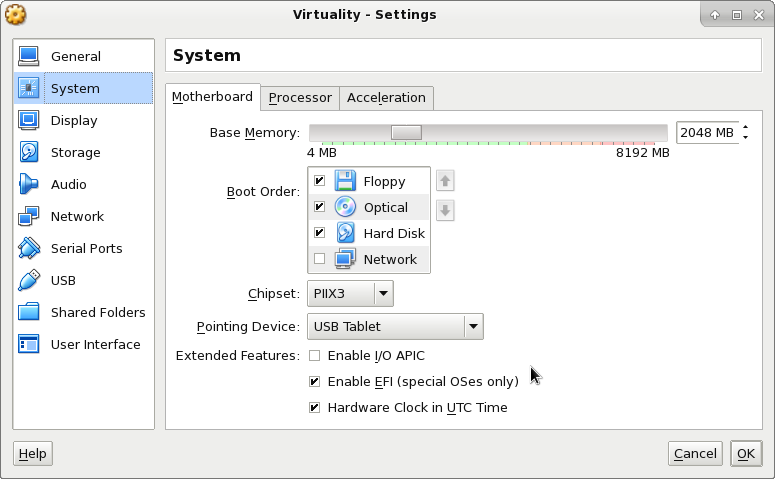
\includegraphics[width=0.8\textwidth]{resin-vbox}
	\caption{Virtualbox general settings for resinOS}
	\label{fig:resingen}
\end{figure}

\begin{figure}
	\centering
	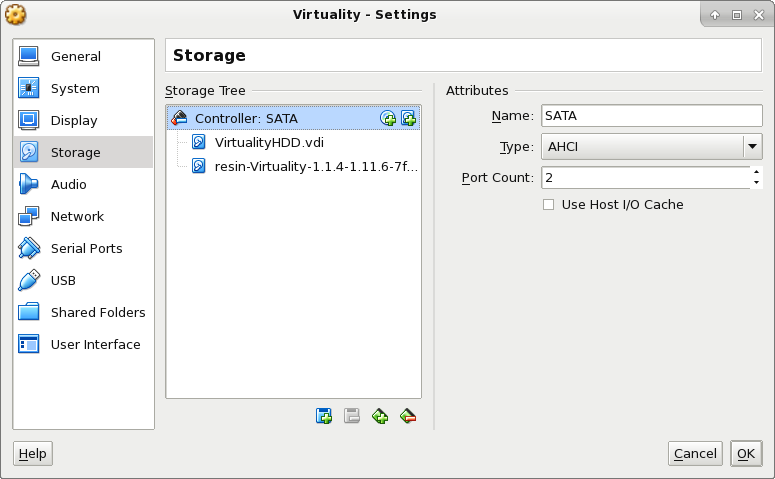
\includegraphics[width=0.8\textwidth]{resin-vbox2}
	\caption{Disk settings for resinOS}
	\label{fig:resindisk}
\end{figure}

To properly connect and download eventual containers we have to configure some forwards. In the ``Network'' menu, select advanced, then Port forward. Configure now the forward of port 8022 to 22  and 2375 to 2375 for client host 10.0.2.15 (usually).

If the virtual machine is run now, the downloaded boot image creates a new instance of resinOS on the previously created virtual drive. The new disk is populates with the settings specified in the configuration step. The system shuts down automatically. Now the resin boot image can be removed.

\subsubsection{Run a Balena container in resinOS}

\textit{resinOS} is shipped with Balena pre-installed and the system is now ready to run any desired container. 
An example application responding to a simple web request can be set-up and tested with the following guide.

Clone the repository to a local directory with
\begin{verbatim}
	git clone https://github.com/resin-io-playground/resinos-sample
\end{verbatim}

Now enter the repository and edit ``Dockerfile''. Replace the text after FROM with \textit{resin/intel-nuc-alpine-node:slim}. Now compile and upload the container to the virtual host with

\begin{verbatim}
	sudo resin local push localhost --source .
\end{verbatim}

Browsing to localhost should now display a test page.

\subsubsection{Evaluation}

The resinOS core ships with an even kernel version. Unfortunately the PREEMPT\_RT patch is not available for odd kernel versions and this image can therefore be patched only manually. This increases the maintenance effort and makes thus a resinOS based approach unpractical.

NOTE: Consider Xenomai patch for this concept

\subsection{Ubuntu core}
{\small\textsc{Test-run Ubuntu core, 25/07/18} \bigskip}

Ubuntu Core is a project to bring small applications to embedded devices based on standard Ubuntu technology. The software is shipped in a snap and run sandboxed in a container like environment while keeping the transparency of a traditional application. 

Snaps are standard feature of Ubuntu based distributions since since 2 years now. It combines the advantages of a package manager and a virtualized container. Even though the snap itself runs on isolated resources provided through proper \texttt{cgroup} configuration, it maintains the accessibility and transparency a locally installed software would have. The running applications are practically sandboxed, having separated partitions for binaries, application specific settings, and the actual file system of the host OS. The host and the binary partitions are read-only, protecting the hosting system from evetualy malicious software. In addition, the binaries are digitally signed and thus avoid tampering with the executables. This gives the flexibility of continuous updates of an application, independent from the host system and flavor, and without interacting with the file system of the host.

A variety of Linux flavors support snaps and snap stores can be privately hosted, making this solution very interesting. More details can be found at \url{https://snapcraft.io/}

In this test a setup is described and feasibility of the candidate is verified.

\subsubsection{Local Virtual machine}

Like in the previous example, the image is downloaded, ready to be used. Visit \url{https://developer.ubuntu.com/core/get-started} for an additional step by step guide.
Get and unpack the latest KVM core image (replace version numbers where appropriate):

\begin{verbatim}
	wget http://cdimage.ubuntu.com/ubuntu-core/16/stable/current/ubuntu-core-16-amd64.img.xz
	unxz ubuntu-core-16-amd64.img.xz
\end{verbatim}

Before it can be used, the image has to be converted from a raw image to a virtual drive. We convert the image again with the Virtualbox CLI tool.

\begin{verbatim}
	VBoxManage convertdd ubuntu-core-16-amd64.img ubuntu-core-16-amd64.vdi
\end{verbatim}

Now we create a new virtual machine, based on Ubuntu 64bit, and add the existing disk. The system is ready to run.

In order to be able to connect to the new virtual machine, we need a Ubuntu one account. In the account we then specify the ssh key we are going to use to connect to the core device. The booted device will ask the email of the Ubuntu one account and downloads the ssh key. Finally to connect via ssh we have to configure some forwards. In the settings, select ``Network'', advanced, then Port forward. Configure now the forward of port 8022 to 22 for client host 10.0.2.15 (usually).

\subsubsection{Evaluation}

Unfortunately, the core is stripped to minimum and thus patching for real-time capabilities is not easily possible. This means, it does not include a package manager and patching the kernel is hard as a patch command not installed.

The core used snaps for applications, thus using snaps for installations was considered. Unfortunately, even though the snap feature is native to Ubuntu, and a patched kernel could reach real-time properties, the binding with the hosts name and file-space hinders the use of application duplicates. This approach is thus archived for the moment.

If all other attempts are not successful enough, a conversion of the apps to snaps and proper configuration might be considered.

\subsection{Ubuntu Server 16.04.4 with xenomai}

{\small\textsc{Testrun Xenomai, 26/07/18} \bigskip}

Xenomai is a os extension to implement POSIX real-time features to a standard kernel. Xenomai supplements it with Cobalt, a small real-time infrastructure which schedules time-critical activities independently from the main kernel logic.The interfacing with an interrupt dispatcher (I-pipe) allows to increase response time and performance and thus enables also for hard-real-time execution. Through extension with skins, also non POSIX compliant real-time software can be configured to run on a Xenomai patched system.

Main concerns of this approach are setup complexity and maintainability.

\subsubsection{Local Virtual machine}
\label{sec:xenoinst}
The os should be lightweight but still fully featured. Thus, an Ubuntu server flavor with minimal installation has been chosen. Download the image from the Ubuntu website \url{http://releases.ubuntu.com/16.04.4/}. The latest patch available for Ubuntu is based on Kernel 4.9.x. Ubuntu 16.04 is the closest version with 4.4.x and thus the candidate for a kernel upgrade.

\begin{verbatim}
	# download image
	wget http://releases.ubuntu.com/16.04.4/ubuntu-16.04.4-desktop-amd64.iso
	# verify image hash
	curl -sfL http://releases.ubuntu.com/16.04.4/SHA256SUMS
	|	sha256sum -c 2>&1 | grep OK
\end{verbatim}

Now we create a new Ubuntu 64bit based virtual machine with a disk size of at least 20GB. We need the space for the compiling of the kernel. Memory size can be arbitrary chosen between 384 mB and $\inf$. When setting the number of assigned CPUs, consider that the more, the faster is the compiling of the new kernel.
Before starting the machine, we add the Ubuntu server disk image to the cd drive of the new machine.

Now follow the guide of the installer. If asked, add only ssh server to the pre-installed packages and continue with software deployment. When installation is done, don't forget to upgrade the system to the newest packages and restart before proceeding with the kernel build. Execute:

\begin{verbatim}
	apt-get update && apt-get dist-upgrade -y
\end{verbatim}

The patching steps have all be resumed in an installer script by Pasquale Antonante. Unfortunately some steps are outdated and some configurations have changed. The script has therefore been updated and placed in the appropriate directory of the repository. The install script provides downloads of the two patches, Xenomai/Cobalt and I-Pipe, the kernel, performs the patch and installs new kernel and the Balena environment.

\subsubsection{Evaluation}

Because of the interrupt handling allowing out-of-band interrupt handlers and thus immediate IRQ reception, Xenomai is a ideal candidate for hard-real-time constraints. The patching is bound to kernel versions, thus the progress depends on the patch development of I-Pipe. Currently the kernel patch is stuck at version 4.14.4.(the latest kernel shipped with Ubuntu 16.04 LTS is 4.15.0-29, the latest stable 4.17.11). The scheduling of the real-time tasks is based on the co-kernel and is thus easier to modify and change, a promising approach.

\subsection{Ubuntu Server 16.04.4 with patch RT}

{\small\textsc{Testrun Preempt-RT, 27/07/18} \bigskip}

The main aim of the PREEMPT\_RT patch is to minimize the amount of kernel code that is non-preemptible. Therefore several substitution mechanisms and new mechanisms are implemented.

\subsubsection{Local Virtual machine}

The same conditions as in the previous example apply. Download the image from the Ubuntu website \url{http://releases.ubuntu.com/16.04.4/}, if not already done. Also here the latest patch available for Ubuntu is based on Kernel 4.9.x. Ubuntu 16.04 is again the closest version with 4.4.x and thus the candidate for a kernel upgrade. See section \ref{sec:xenoinst}.

The patching steps have all be resumed in an installer script similar to the previous. The install script provides downloads of the patch and the kernel, performs the patch and installs new kernel and the Balena environment.

%downloaded patched kernel from kernel.org
%make menuconfig
%-> (needs libncurses5 libncurses5-dev)
%remove cpu-freq and cpu idle (needs PM cpu deactivation first)

For further guides on how to compile and install a kernel, visit \url{ https://medium.freecodecamp.org/building-and-installing-the-latest-linux-kernel-from-source-6d8df5345980}

\subsubsection{Evaluation}

The Preempt-RT requires a dedicated patch and recompiling of the kernel to support soft-real-time properties. The additional slicing preformed to the kernel tasks allows faster preemption and a better control of the CPU scheduling. Compared to the previous example, the handling of interrupt flow can not be controlled to the same extend reaching thus a lower level of real-time feasibility. Lately the project has made remarkable progress. To exploit its full potential, an Ubuntu 18.04 LTS kernel patching as a future step is taken into consideration.

\section{Tests of system}

{\small\textsc{Testrun and comparison of systems, 30/07/18} \bigskip}

Some small cyclic execution tests are performed to verify default availability of real-time sheduling and the timing behavior of the scheduler.

\subsection{rt-tests}

the rt-tests suite includes a list of small tool binaries which may be used to test properties of real-time systems. The most prominent are \textit{cyclictest} and \textit{hackbench}. To install the software we may use one of the two approaches:

1) We use Xenomai, thus there is a tool package ready and available

\begin{verbatim}
	apt-get install xenomai-system-tools
\end{verbatim}

2) We use another real-time approach and compile the binaries from the source code.
For this approach we need first some additional packages. Get them with:

\begin{verbatim}
	sudo apt-get install build-essential libnuma-dev
\end{verbatim}

Now proceed with the installation. Download the git repository and compile the source.

\begin{verbatim}
	git clone git://git.kernel.org/pub/scm/utils/rt-tests/rt-tests.git
	cd rt-tests
	git checkout stable/v1.0
	make all
	make install
\end{verbatim}

The last step is optional. The binaries can now be run (within the directory) to perform the different tests. An example of a test, as recommended on Kernel.org is: 

\begin{verbatim}
	cyclictest -t 50 -i 1000 -d 86400 -l 10000000 -a -p 99 -n
\end{verbatim}

The code in the example creates fifty tasks with priority 99 (maximum) an intervall of 1000 $\mu s$ and a task delay of 86400 $\mu s$ and using a clock-based nanosecond timer. There is a difference between normal and patched images, but the actual values are for now far from ideal. At the moment, as the host is not real-time capable, the delays also depend on the scheduling of the host which sets up the virtual machine. 

\subsection{Other testing tool}

A list of other tools that might be helpful:

\begin{itemize}
	\item \textbf{htop} a colored memory view to analyse memory use of single processes
	\item \textbf{iftop} interface monitor to view actual network traffic
	\item \textbf{iotop} generic i/o monitor
\end{itemize}

\section{Additional fixes}

balena, even though installed via script, is not properly configured

\url{https://docs.docker.com/install/linux/linux-postinstall/#configuring-remote-access-with-systemd-unit-file}


\section{Issues and verifications}

{\small\textsc{, 31/07/18} \bigskip}



\begin{figure}
	\centering
	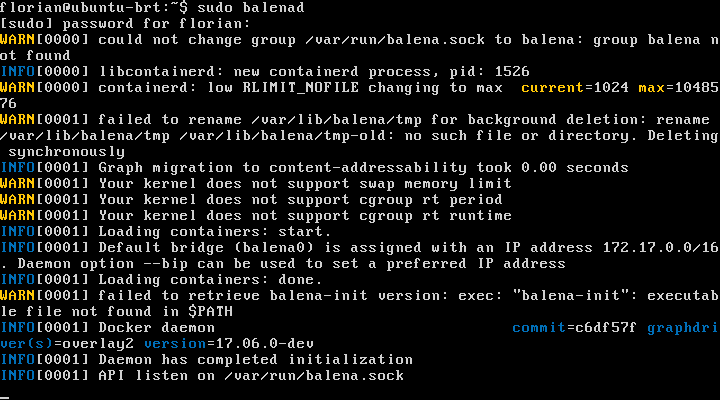
\includegraphics[width=0.8\textwidth]{balena-err}
	\caption{text}
\end{figure}

WARN[0001] Your kernel does not support swap memory limit 

Oh nuts, is it...

\#CONFIG\_MEMCG\_SWAP\_ENABLED is not set -> WARNING: No swap limit support

and

\# CONFIG\_MEMCG\_KMEM is not set -> WARNING: No memory limit support

possible temporary fix https://github.com/moby/moby/issues/4250



WARN[0001] Your kernel does not support cgroup rt period 
WARN[0001] Your kernel does not support cgroup rt runtime 
-> not activated if Preempt full!!

\section{Virtualization sustainability tests}

{\small\textsc{Testrun Containers \& CPU pinning, 01/08 - 3/08/18} \bigskip}

% AWS ? virtual machine test resoure pinning in vbox -> pin local host? balance share.


man 7 capabilities  -> list of all linux based capabilities


--> check sourcecode of balena tells the compose supported commands and capabilities. Balena sourcecode declarations differ from the one on the docker site.

creation of a balena container for RT tests
-> resin.io
Documentation describes that balena containers for resinOS (And thus also for other balena systems), need a local docker-compose installation and upload via remote.


\section{Meetings}

\begin{table}[h]
	\centering
	\caption{List of meetings during the stay at UC Berkeley}
	
	\begin{tabular}{l p{5cm} p{5cm}}
	Date & Participants & Topics \\
	\hline
	26/07/18 & Martin Sehr, Ines Ugalde Diaz, Antonio Iannopollo, Florian Hofer & Project setup, generic requirements, questions for BU\\
	31/07/18 & Martin Sehr, Ines Ugalde Diaz, Florian Hofer & Progress of testing, Dummy testing approach\\
	07/08/18 & Ines Ugalde Diaz, Florian Hofer & \\
	10/08/18 & Ines Ugalde Diaz, Florian Hofer & \\
	\hline
	\end{tabular}
	
	\label{tab:meeting}
\end{table}

\end{document}


% Fri Non slide 



